% !TeX spellcheck = en_US
\chapter{Experiments in Simulation}\label{ch:sim}%

This chapter reports the simulation experiments. Section~\ref{sec:sim-setup} fixes the experimental setup. Section~\ref{sec:sim-teacher} reports the training of the privileged teachers and the negative results on end-to-end threading that motivated the hybrid teacher. Section~\ref{sec:sim-student} reports the main student ablations in simulation, Section~\ref{sec:sim-design} the design ablations of the student, and Section~\ref{sec:sim-online} the online distillation baselines. Section~\ref{sec:sim-inventory} inventories every ablation that the code base supports and marks which of them have results. Numbers that are not yet available are marked \tbd{} and listed in the draft to-do file.

\section{Experimental Setup}\label{sec:sim-setup}

All simulation experiments use the system of Section~\ref{sec:system} in Isaac~Sim~5.1 with physics at 120\,Hz and control at 15\,Hz, on a single NVIDIA GeForce RTX~5090. Teachers are trained with 512 parallel environments for 200 epochs, which takes about ten hours per teacher; the student is trained offline for 300 epochs in about 30 minutes. The student data set is the one of Section~\ref{sec:dataset}: 20 successful ten-cycle demonstrations of the M24 hexagonal nut collected from 32 environments with 30 random arm impulses each, 19\,486 frames in total, under lighting and texture randomization of the dome light, the tabletop, the nut and bolt textures, the floor texture, and the image background in the style of DextrAH-RGB~\cite{Singh2025}. Figure~\ref{fig:sim-scenes} shows the parallel training scenes and the randomized student views. Unless stated otherwise, students use the Cartesian action contract with $H=8$, sixteen Euler steps, a temporal-ensemble decay of 0.5, EMA weights, and the DP3-style encoder; evaluation follows Section~\ref{sec:evaluation} with ten trials of ten cycles on the M24 nut in a nominal scene without physical domain randomization.

\begin{figure}[htb]%
    \centering%
    \begin{subfigure}[b]{0.48\textwidth}
        \centering
        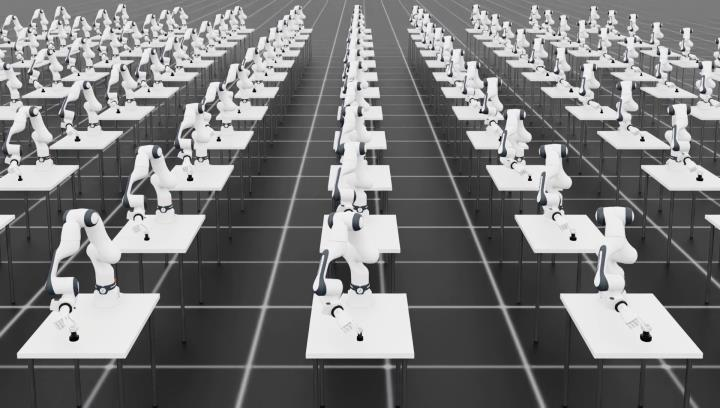
\includegraphics[width=\textwidth]{figures/nuts/sim_parallel_training.png}
        \caption{Parallel teacher-training environments.}
    \end{subfigure}\hfill
    \begin{subfigure}[b]{0.48\textwidth}
        \centering
        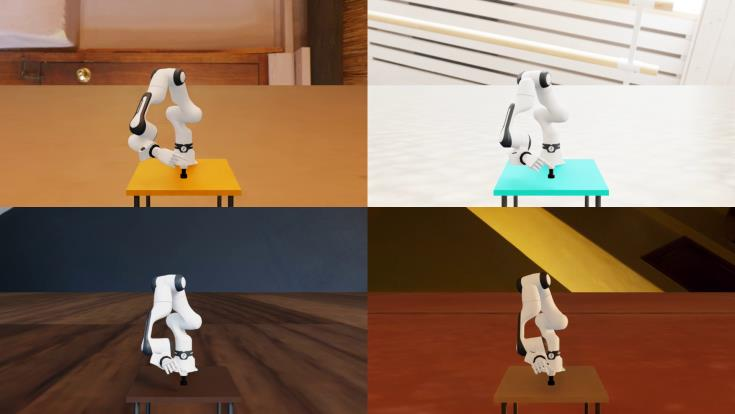
\includegraphics[width=\textwidth]{figures/nuts/sim_visual_randomization.png}
        \caption{Lighting and texture randomization.}
    \end{subfigure}\\[2mm]
    \begin{subfigure}[b]{\textwidth}
        \centering
        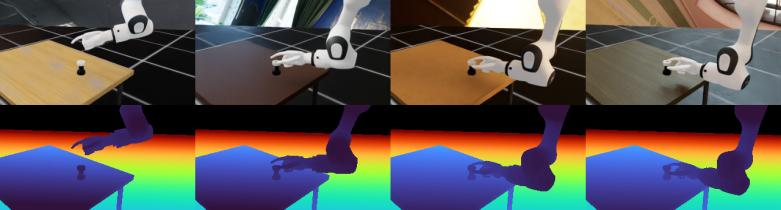
\includegraphics[width=\textwidth]{figures/nuts/student_rgbd_randomized.png}
        \caption{Student RGB (top) and depth (bottom) observations under visual randomization.}
    \end{subfigure}
    \caption{Simulation scenes. Teacher policies are trained in hundreds of parallel workcells; demonstrations for the student are rendered with randomized dome lighting, table, object, floor, and background textures, from which the student sees aligned RGB and depth. Images reproduced from the accompanying paper~\cite{NUTS2026}.}%
    \label{fig:sim-scenes}%
\end{figure}%

\section{Teacher Training}\label{sec:sim-teacher}

\subsection{End-to-End Threading Does Not Train}\label{sec:sim-e2e}

The first design of this project, laid out in the exposé, trained a single PPO policy to acquire a pinch grasp and thread a nut on faithfully simulated SDF threads. Over more than forty reward and controller variants on two robot platforms, this did not yield a usable threading policy, and the pattern of failures is informative. With the nut pre-seated in the pinch and the thread modeled by SDF colliders, a policy reached about 85\,\% of a geometric success criterion, but replay showed that the criterion was satisfied by pressing the nut axially through the thread body rather than by turning it; every attempted remedy, including lower depenetration velocities, alignment-gated descent rewards, contact-force penalties, and cumulative-advance gates, either reopened the exploit or removed the descent gradient entirely. With the nut spawned free on the bolt, the pinch itself became the obstacle: the policy either batted the nut off its spawn or hovered in an aligned pose without closing, because the shaped approach reward paid out before any contact was established. With helical waypoint tracking rewards ported from SimToolReal~\cite{Kedia2026}, grasps survived but the nut never wound onto the thread. The conclusion drawn from these experiments is twofold. A reward that simultaneously shapes grasp acquisition, grasp retention, helical progress, and clean termination over a multi-cycle horizon could not be found by iteration, and the SDF thread contact offered the policy a cheaper solution than threading. Both problems are removed by the design of Chapter~\ref{ch:method}: the simplified thread model makes axial progress a kinematic consequence of rotation, and the hybrid teacher assigns the transition phases, which are easy to script but hard to reward, to scripted controllers.

\subsection{Threading and Pickup Experts}\label{sec:sim-experts}

With the simplified thread model and the three-stage reward of Section~\ref{sec:teacher}, the threading expert learns the single $60\degree$ turn from the engaged nut. On the Tiangong\,2 platform the recipe with the $\pm30\degree$ initial-yaw curriculum reached a population success rate of 83.6\,\% at the end of training with a peak of 90.0\,\%; on the FR3 platform the retained M24 teacher, trained for 200 epochs with the curriculum and the axial-height randomization, completed ten consecutive cycles in all 32 hybrid-teacher candidate environments without a single transition failure, which is the property that matters for demonstration generation. Table~\ref{tab:teacher-results} summarizes the teacher results; the single-turn success rate of the FR3 teacher at the final curriculum level is \tbd.
% TODO(results): report final-epoch single-turn success and curriculum level of the retained FR3 M24 threading teacher (TensorBoard of the run promoted on 2026-09-10) and of the M24/M30/M36 multi-size teacher.

\begin{table}[htb]%
    \centering%
    \caption{Teacher training results. Success is the population success rate at the end of training; the hybrid-teacher column counts candidate environments that completed the required cycles with zero transition failures.}%
    \label{tab:teacher-results}%
    \resizebox{\textwidth}{!}{%
\begin{tabular}{llccc}
        \toprule
        Teacher & Platform & Success & Peak success & Hybrid rollout \\
        \midrule
        Threading, $\pm30\degree$ yaw curriculum & Tiangong\,2 & 83.6\,\% & 90.0\,\% & -- \\
        Threading, M24, yaw and depth randomization & FR3 & \tbd & \tbd & 32/32 ten-cycle \\
        Threading, M24/M30/M36 one-hot & FR3 & \tbd & \tbd & \tbd \\
        Pickup and engagement & Tiangong\,2 & 0\,\% (G1) & -- & -- \\
        Pickup and engagement & FR3 & 0\,\% (G1) & -- & -- \\
        \bottomrule
    \end{tabular}}
\end{table}%

The pickup expert is the weak link of the full-task variant. On both platforms it learned to approach, pinch, and lift the loose nut, with 95.3\,\% grasp and 94.5\,\% lift success on Tiangong\,2 and 99.8\,\% pinch success on the FR3, but it did not learn the terminal engagement: the aligned handoff above the bolt tip within 10\,mm and the engagement within 5\,mm held for ten steps were reached in 0\,\% of episodes. Reward variants that added hold-or-drop terms, velocity brakes, goal-gated drop penalties, and disturbance curricula changed the grasp and lift conversion but not the terminal success. The threading results of this thesis therefore start from an engaged nut, and nut engagement is left to future work (Chapter~\ref{ch:conclusion}).

A teacher was also trained under the hardware-matched libfranka-style Cartesian impedance controller with the published example gains (150\,N/m, 10\,N\,m/rad, 20\,N\,m/rad nullspace) instead of the Factory gains. Over 200 epochs the grasp-center distance fell from 180\,mm to a minimum of 38\,mm, but neither fingertip entered the 10\,mm face tolerance, the perpendicular-pinch fraction decreased from 73\,\% to 22\,\% over training, and contact, grasp, turn, and success metrics remained zero throughout. Cartesian tracking error stayed near 25\,mm under this controller, and the action-bound loss grew late in training, which indicates saturated commands. The finding is that the softer gains, not the reward, prevent the policy from reaching contact, and the reported teachers therefore keep the Factory gains in simulation while the physical controller is matched to them (Chapter~\ref{ch:real}).

\section{Student Ablations in Simulation}\label{sec:sim-student}

The main ablation study addresses the four questions of Section~\ref{sec:research-questions}: (Q1) whether a unified multi-cycle student outperforms repeated execution of a single-cycle policy, (Q2) the contribution of the point-cloud encoder, (Q3) the effectiveness of flow matching relative to deterministic behavior cloning with LSTM and Transformer backbones, and (Q4) the benefit of augmenting simulation demonstrations with human-corrected real-world trajectories. Six students are compared under matched training and evaluation budgets, changing only the component named by each ablation.

\begin{enumerate}
  \item[(a)] \emph{Single-cycle student.} Trained on real-world-augmented single-cycle demonstrations and invoked ten times, with its temporal context reset after each cycle.
  \item[(b)] \emph{ResNet visual encoder.} The DP3 encoder is replaced by the one-branch, ImageNet-pretrained ResNet-18 stage-2 encoder that fuses RGB, log depth, validity, and calibrated XYZ geometry into a 64-D feature; policy, objective, data, and budget are unchanged.
  \item[(c)] \emph{DP3 vision with LSTM regression.} The flow-matching Transformer is replaced by the DextrAH-RGB-style backbone, a layer-normalized 512-unit LSTM followed by a 512--512--256 ELU MLP, trained by deterministic supervised action regression on the same data.
  \item[(d)] \emph{DP3 vision with Transformer regression.} The deterministic ACT-style Transformer of Section~\ref{sec:baselines} with eight learned action queries predicts the eight-step chunk.
  \item[(e)] \emph{Simulated data only.} The multi-cycle flow student is trained on simulated hybrid-teacher demonstrations alone, excluding the human-corrected real-world data.
  \item[(f)] \emph{Full method.} One flow-matching student trained on complete multi-cycle hybrid-teacher demonstrations augmented with human-corrected real-world data.
\end{enumerate}

Table~\ref{tab:ablation-sim} reports the simulation results on the M24 hexagonal nut. The unified multi-cycle student (f) completes all ten cycles in every trial, whereas the single-cycle student (a) completes 5.5 cycles on average; its typical failure is that it slips off the edge of the nut after a few cycles, because it learned the basic threading skill but not to follow the axial advance of the nut, which a policy that only ever saw one cycle has no reason to represent (Q1). Both deterministic regression heads fail: the LSTM backbone (c) diverges before completing a single cycle, and the Transformer backbone (d) survives slightly longer, with 1.4 cycles on average and a large positive cyclic error, before the same compounding-error problem ends the trial (Q3). Neither (c) nor (d) was advanced to hardware testing. The student trained on simulated data alone (e) performs perfectly in simulation and even reaches a smaller cyclic error and deviation than the full method, which is expected because (e) is evaluated on the distribution it was trained on, whereas (f) also absorbs real-world corrections that the simulator does not require; the value of (f) appears only on hardware (Chapter~\ref{ch:real}).

\begin{table}[htb]%
    \centering%
    \caption{Simulation ablations on the M24 hexagonal nut over ten trials. Each defined entry reports mean $\pm$ standard deviation. Completed cycles are averaged across trials, cyclic-error statistics use completed cycles only, and the ten-cycle error compares the accumulated rotation with the $600\degree$ target; it is reported as ``--'' when no trial completes all ten cycles. Errors are signed in degrees: negative denotes lag and positive overshoot. Results from the accompanying paper~\cite{NUTS2026}.}%
    \label{tab:ablation-sim}%
    \small
    \begin{tabular}{lccc}
        \toprule
        Ablation & Completed cycles $\uparrow$ & Cyclic error $\rightarrow0$ & Ten-cycle error $\rightarrow0$ \\
        \midrule
        (a) single-cycle student & $5.5\pm0.8$ & $-4.16\pm3.21$ & -- \\
        (b) ResNet encoder & $2.3\pm0.9$ & $+20.17\pm7.80$ & -- \\
        (c) DP3 + LSTM regression & $0.0\pm0.0$ & -- & -- \\
        (d) DP3 + Transformer regression & $1.4\pm0.8$ & $+124.21\pm18.50$ & -- \\
        (e) simulated data only & $10.0\pm0.0$ & $-1.77\pm1.02$ & $-17.7\pm3.23$ \\
        (f) full method & $10.0\pm0.0$ & $-2.13\pm1.10$ & $-21.30\pm3.48$ \\
        \bottomrule
    \end{tabular}
\end{table}%

For Q2, the vision encoders are compared both through the closed-loop ablation (b) and through a representation probe. A shared pose decoder is trained on the frozen visual feature of each encoder to predict the nut position and orientation. The DP3 feature yields a position error of 8\,mm and a rotation error of $15.16\degree$ in simulation, whereas the ResNet feature yields a similar position error of 8.6\,mm but a notably higher rotation error of $31.20\degree$. In closed loop the ResNet student (b) completes 2.3 cycles with a large positive cyclic error, against ten for the DP3 student. The substantially larger rotational prediction error of the image-space representation suggests that it is less effective at preserving the geometry required for repeated re-grasping under viewpoint and axial change, which is exactly what the cyclic task demands.

\section{Design Ablations of the Student}\label{sec:sim-design}

The ablations of Section~\ref{sec:sim-student} compare the final student against alternatives at the level of the paper. The design of the student itself was fixed by a sequence of controlled single-rollout ablations on six-cycle sequential-threading data, which this section reports because they document why each component is present. All runs in this section use the privileged 6-D nut-pose observation or the RGB-D observation as stated, 20 impulse-augmented demonstrations, 300 epochs, the Cartesian contract, $H=8$, and the student-owned cyclic evaluation with a six-cycle requirement at a fixed seed; they are matched single rollouts, not success rates.

\subsection{Action Contract}\label{sec:sim-contract}

The first offline flow students used the 17-D joint-PD contract on pickup demonstrations. With privileged 6-D observations they reached a training flow loss of 0.03 and an offline teacher-fit chunk RMSE of 0.040 with correlation 0.998, but in closed loop they held a proper grip for about 1.3\,s, lifted the nut by up to 10.5\,cm, and then released it before the handoff goal; the best handoff distance was 36\,mm against a 10\,mm tolerance, and no trial succeeded. Terminal-hold padding of the training windows lengthened grip retention slightly and moved the closest approach by 5\,mm but did not change the outcome. A residual variant that predicts arm-position residuals instead of absolute references was numerically stable but did not grasp at all. The same demonstrations materialized in the native Cartesian contract produced, with the same student, 10/10 grasps and lifts, 5/10 terminal successes on the handoff-only task, and 8/10 qualified handoffs, 7/10 engagement entries, and 2/10 held engagements on the stricter engagement task. On the full-task demonstrations with the joint-PD contract, both a privileged and an RGB-D student that reproduced their labels offline diverged within the first half second of closed-loop control and achieved 0\,\% pickup, with controlled-joint RMSE of $14\degree$ and $27\degree$, respectively, against the nominal trajectory. These results, together with the zero-order-hold argument of Section~\ref{sec:action-contract}, fixed the Cartesian contract for all later students. Table~\ref{tab:contract} summarizes them.

\begin{table}[htb]%
    \centering%
    \caption{Action-contract ablation of the offline flow student on pickup demonstrations (privileged 6-D observation, single seed). G0 is the handoff waypoint above the bolt tip and G1 the engagement goal.}%
    \label{tab:contract}%
    \resizebox{\textwidth}{!}{%
\begin{tabular}{llcccc}
        \toprule
        Contract & Task & Grasp & Lift & G0 & G1 held \\
        \midrule
        17-D joint-PD, absolute & engagement & 10/10 & 10/10 & 0/10 & 0/10 \\
        17-D joint-PD, terminal padding & engagement & 10/10 & 10/10 & 0/10 & 0/10 \\
        10-D joint-PD, residual & engagement & 0/10 & 0/10 & 0/10 & 0/10 \\
        9-D Cartesian (native) & handoff only & 10/10 & 10/10 & 5/10 & -- \\
        9-D Cartesian (native) & engagement & 10/10 & 10/10 & 8/10 & 2/10 \\
        \bottomrule
    \end{tabular}}
\end{table}%

\subsection{Progress and Phase Conditioning}\label{sec:sim-conditioning}

On six-cycle sequential-threading demonstrations with policy-only impulses, a state-conditioned flow student completed four cycles and failed the physical return of the fifth with a 141\,mm position residual, although its offline fit was excellent (first-action RMSE 0.005). With impulses in every phase segment and the global trajectory progress $p_t$ added to the condition, the student completed all six required cycles in 735 control ticks with zero transition failures; its release times, however, drifted increasingly behind the teacher, by $+8.6$\,s at the sixth release, and the fifth cycle took twice as long as the others. Adding the three-way process-phase encoding reduced the completion time to 609 ticks, equalized the cycle durations to 6.7 to 7.1\,s, reduced the release-time errors against the teacher to within $\pm0.5$\,s, reduced the controlled-joint RMSE against the nominal trajectory from $11.5\degree$ to $4.7\degree$ and the TCP position RMSE from 75\,mm to 28\,mm, and reduced the final cumulative nut-turn error from $-60\degree$ to $-8\degree$. The offline teacher-fit of the phase-conditioned checkpoint was marginally worse than that of the progress-only checkpoint (first-action RMSE 0.0046 against 0.0044), so the closed-loop improvement is not explained by a better fit; the phase encoding acts as a synchronization signal that keeps the student's internal clock aligned with physical events when the cycle duration deviates from nominal. Both conditions have been enabled by default since. Table~\ref{tab:conditioning} collects the numbers.

\begin{table}[htb]%
    \centering%
    \caption{Conditioning ablation on six-cycle sequential threading (privileged 6-D observation, matched single rollouts at one seed). RMSE values are against the nominal teacher trajectory in absolute time; the final turn error is the cumulative nut-rotation error after the last cycle.}%
    \label{tab:conditioning}%
    \resizebox{\textwidth}{!}{%
\begin{tabular}{lcccc}
        \toprule
        Condition & Cycles & Ticks & Joint RMSE & Final turn error \\
        \midrule
        state only, policy-only impulses & 4/6 & 776 & $14.9\degree$ & -- \\
        state + progress $p_t$, all-phase impulses & 6/6 & 735 & $11.5\degree$ & $-60.3\degree$ \\
        state + progress + phase $\vec{e}^{m}_t$ & 6/6 & 609 & $4.7\degree$ & $-8.2\degree$ \\
        \bottomrule
    \end{tabular}}
\end{table}%

\subsection{Vision Encoder and Pretraining}\label{sec:sim-vision}

The first RGB-D student used the two-branch cross-attention encoder with an auxiliary nut-position head and completed all six cycles in 617 ticks, matching the privileged student; a recollection with explicit success markers and retraining reproduced the result in 627 ticks. Initializing the DP3 encoder from a pose-regression pretraining on full-task images and fine-tuning it jointly with the flow objective did not help: the student completed three cycles and lost the grip in the fourth, and a pose-retention probe showed that joint training had moved the latent coordinate system so that the pretrained 6-D decoder no longer applied, while the jointly trained position head still achieved 0.37\,mm. Pretraining the DP3 encoder on rendered sweeps of a free-moving nut from the calibrated camera reached a held-out position error of 5.9\,mm and a hexagon-symmetry-aware rotation error of $46\degree$; fine-tuning on hybrid-teacher images with phase-balanced sampling reached 1.9\,mm and $3.8\degree$ on held-out teacher episodes, and 2.8\,mm and $6.6\degree$ on images from a student rollout, with the largest errors during grasp occlusion in pickup. The ten-cycle DP3 student of Table~\ref{tab:ablation-sim} was initialized from the sweep-pretrained encoder with all encoder parameters trainable; it completed all ten cycles in 1072 ticks with a maximum turn of $60.3\degree$, a mean release-time lag of 2.7\,s against its source demonstration that reached 7.4\,s by the tenth cycle, and a mean absolute retained-turn error of $3.1\degree$, which indicates timing drift rather than lifecycle failure. A closed-loop comparison of the DP3, Adapt3R-style, and ResNet encoders under identical data and budget beyond ablation (b) is \tbd{} (Table~\ref{tab:encoders}).
% TODO(results): train offline_flow_matching_adapt3r_agent.yaml and the one-channel ResNet encoder on the ten-cycle M24 dataset with the same recipe as the DP3 student; evaluate ten trials each.

\begin{table}[htb]%
    \centering%
    \caption{Vision-encoder ablation of the flow student on the ten-cycle M24 task (ten trials). The DP3 row is the full method; the remaining rows are placeholders.}%
    \label{tab:encoders}%
    \resizebox{\textwidth}{!}{%
\begin{tabular}{lccc}
        \toprule
        Encoder & Completed cycles $\uparrow$ & Cyclic error $\rightarrow0$ & Ten-cycle error $\rightarrow0$ \\
        \midrule
        DP3 point cloud (RGB + XYZ) & $10.0\pm0.0$ & $-2.13\pm1.10$ & $-21.30\pm3.48$ \\
        ResNet-18 early fusion (b) & $2.3\pm0.9$ & $+20.17\pm7.80$ & -- \\
        Adapt3R-style (frozen ResNet + 3D attention) & \tbd & \tbd & \tbd \\
        Two-branch cross-attention RGB-D & \tbd & \tbd & \tbd \\
        Depth-only CNN & \tbd & \tbd & \tbd \\
        \bottomrule
    \end{tabular}}
\end{table}%

\subsection{Privileged Observations, Horizon, Integration Steps, and Inputs}\label{sec:sim-sweeps}

The privileged observation modes serve as upper bounds and as diagnostics: with the nut position (3-D) or pose (6-D) appended to the proprioception instead of the visual feature, the same flow student is trained and evaluated without rendering. On six-cycle sequential threading the privileged 6-D student and the RGB-D student both completed six cycles at matched settings, which shows that the visual feature carries the information the task needs. The remaining sweeps over the action horizon $H$, the number of Euler steps $N$, the temporal-ensemble decay, the hand-velocity input, and the terminal-hold padding are implemented as command-line options of the offline trainer and evaluator but have not been run as controlled studies; Table~\ref{tab:sweeps} gives the skeleton.
% TODO(results): run action-horizon sweep (H in {1, 4, 8, 16}), ODE-step sweep (N in {1, 4, 8, 16, 32}), temporal-ensemble decay in {0, 0.5, 0.8}, and --hand-velocity-observation omitted on the ten-cycle M24 dataset; ten trials each; also record inference latency per N.

\begin{table}[htb]%
    \centering%
    \caption{Student hyperparameter sweeps on the ten-cycle M24 task (ten trials). All cells are placeholders except the reference row.}%
    \label{tab:sweeps}%
    \resizebox{\textwidth}{!}{%
\begin{tabular}{llccc}
        \toprule
        Sweep & Value & Completed cycles $\uparrow$ & Cyclic error $\rightarrow0$ & Latency \\
        \midrule
        reference & $H=8$, $N=16$, decay 0.5 & $10.0\pm0.0$ & $-2.13\pm1.10$ & \tbd \\
        horizon $H$ & 1 / 4 / 16 & \tbd & \tbd & \tbd \\
        Euler steps $N$ & 1 / 4 / 8 / 32 & \tbd & \tbd & \tbd \\
        ensemble decay & 0 / 0.8 & \tbd & \tbd & -- \\
        hand velocities omitted & 26-D proprioception & \tbd & \tbd & -- \\
        privileged 3-D / 6-D nut pose & no vision & \tbd & \tbd & -- \\
        \bottomrule
    \end{tabular}}
\end{table}%

\subsection{Nut-Size Conditioning, Domain Randomization, and Force Observations}\label{sec:sim-robustness}

Three further ablations are implemented but not yet qualified in simulation. The multi-size teacher conditions on a one-hot code of M24, M30, and M36 with round-robin assignment and per-size meshes, keypoints, and pitches; the student is trained on hexagonal nuts of all three sizes without an explicit size input and must infer the size from the point cloud. Per-size simulation results of the student are \tbd; the hardware results across sizes are reported in Chapter~\ref{ch:real}. Physical domain randomization of mass, friction, controller gains, and reset pose is enabled during teacher training and disabled during demonstration collection and evaluation; its effect on the student when enabled at evaluation time is \tbd. Hardware-equivalent force observations, the thumb and index flexion forces projected onto the pad normals and the seven arm joint reaction torques normalized by the FR3 limits, are implemented as observation channels for both teacher and student, but are not yet part of any trained contract; their effect is \tbd. Table~\ref{tab:robustness} lists the skeleton.
% TODO(results): (i) per-size ten-trial evaluation of the multi-size student in simulation; (ii) evaluation with --enable-domain-randomization; (iii) teacher and student retrained with the fingertip-force and joint-torque channels enabled in the actor/student vectors.

\begin{table}[htb]%
    \centering%
    \caption{Robustness ablations in simulation (ten trials of ten cycles). All cells are placeholders.}%
    \label{tab:robustness}%
    \resizebox{\textwidth}{!}{%
\begin{tabular}{llccc}
        \toprule
        Ablation & Condition & Completed cycles $\uparrow$ & Cyclic error $\rightarrow0$ & Ten-cycle error $\rightarrow0$ \\
        \midrule
        nut size & M24 / M30 / M36 & \tbd & \tbd & \tbd \\
        physical DR at evaluation & off / on & \tbd & \tbd & \tbd \\
        force observations & none / fingertip / fingertip + torque & \tbd & \tbd & \tbd \\
        axial-height curriculum & 20\,mm / \tbd & \tbd & \tbd & \tbd \\
        \bottomrule
    \end{tabular}}
\end{table}%

\section{Online Distillation Baselines}\label{sec:sim-online}

Online DAgger was evaluated with the recurrent LSTM student on cyclic threading from privileged 6-D observations under the Cartesian contract, with the hybrid teacher as the label source and a ten-cycle cap per episode. Three intervention schedules were compared. With full teacher control ($\beta=1$), the student learned the first threading turn but not the cyclic release and return motion, because it never controlled a transition and the recurrent state it accumulated under teacher control did not transfer. With full student control ($\beta=0$) and the teacher used only for labels, the student learned the first turn and the complete release-and-return transition, but subsequent turns failed, because the student rarely reached a well-formed re-grasp from which the teacher's turn label was reachable. With a scheduled intervention that decays linearly from full teacher to full student control, the student learned the transition motion and progressed farther: its best checkpoint completed two uninterrupted student-only turn-release-return cycles and entered the third threading attempt, where it lost the proper grip and terminated. SafeDAgger intervention with the thresholds of Section~\ref{sec:online-flow} did not complete a single turn. The earlier full-task LSTM student with the joint-PD contract reported 0\,\% pickup, threading entry, and task success, with 81\,\% of its arm targets saturated at the best-loss checkpoint, which is the student-induced state distribution rather than a controller deficiency, since the same converted commands replay accurately. The online flow-matching student of Section~\ref{sec:online-flow} is implemented with the same hybrid teacher and the Cartesian contract, but no successful student rollout has been demonstrated for it; its result on the cyclic task is \tbd. Table~\ref{tab:online} summarizes the online baselines against the offline students.
% TODO(results): train online_dagger_flow_matching on cyclic_threading with nut_pose_6d (beta=1, H=8) and evaluate ten trials; then the vision variant.

\begin{table}[htb]%
    \centering%
    \caption{Online distillation baselines on cyclic threading (privileged 6-D observation, Cartesian contract). Cycles are student-only completed cycles of the best retained checkpoint in one evaluation rollout; the offline rows are matched single rollouts from Section~\ref{sec:sim-design}.}%
    \label{tab:online}%
    \resizebox{\textwidth}{!}{%
\begin{tabular}{llcc}
        \toprule
        Student & Intervention & Completed cycles & Note \\
        \midrule
        online DAgger LSTM & $\beta=1$ & 0 & learns the turn, not the transition \\
        online DAgger LSTM & $\beta=0$ & 1 & learns the transition, second turn fails \\
        online DAgger LSTM & $\beta$ decayed $1\rightarrow0$ & 2 & grip lost in the third attempt \\
        online DAgger LSTM & SafeDAgger 0.10/0.075 & 0 & no complete turn \\
        online DAgger flow, $H=8$ & $\beta=1$ & \tbd & no qualified rollout yet \\
        offline flow, state + progress + phase & -- & 6/6 & Table~\ref{tab:conditioning} \\
        offline flow, RGB-D & -- & 10/10 & Table~\ref{tab:ablation-sim} \\
        \bottomrule
    \end{tabular}}
\end{table}%

Table~\ref{tab:ladder-results} places several students on the first rung of the evaluation ladder next to their closed-loop outcome. Every listed checkpoint reproduces its training labels with first-action RMSE below 0.04 in normalized action units and correlation above 0.99, including every checkpoint that fails in closed loop. The offline fit is therefore a necessary diagnostic, which rejected no checkpoint in this project, and not a predictor of task success; the closed-loop column is decided by the contract, the conditioning, and the data, not by the fit.

\begin{table}[htb]%
    \centering%
    \caption{Offline teacher-fit against closed-loop outcome for offline flow students (EMA weights, sixteen Euler steps, one training episode). RMSE values are in the student's action units; the joint-PD rows are in physical units, the Cartesian rows in normalized action units.}%
    \label{tab:ladder-results}%
    \resizebox{\textwidth}{!}{%
    \begin{tabular}{llcccl}
        \toprule
        Student & Data & First-action RMSE & Chunk RMSE & Correlation & Closed loop \\
        \midrule
        joint-PD, 6-D nut pose & pickup, 20 episodes & 0.035 & 0.040 & 0.998 & 0/10 handoff \\
        Cartesian, 6-D nut pose, state only & 6-cycle threading, policy impulses & 0.0050 & 0.0110 & 0.9996 & 4/6 cycles \\
        Cartesian, 6-D nut pose, + progress & 6-cycle, all-phase impulses & 0.0044 & 0.0122 & 0.9997 & 6/6 cycles \\
        Cartesian, 6-D nut pose, + progress + phase & 6-cycle, all-phase impulses & 0.0046 & 0.0129 & 0.9997 & 6/6 cycles \\
        Cartesian, RGB-D two-branch, + aux.\ head & 6-cycle, all-phase impulses & 0.0044 & 0.0055 & 0.9997 & 6/6 cycles \\
        Cartesian, DP3 from full-task pretraining & 6-cycle, all-phase impulses & 0.0053 & 0.0105 & 0.9995 & 3/6 cycles \\
        Cartesian, DP3 from sweep pretraining & 10-cycle, all-phase impulses & 0.019 & 0.019 & 0.994 & 10/10 cycles \\
        \bottomrule
    \end{tabular}}
\end{table}%

The pattern across schedules is that decreasing teacher intervention improves long-horizon state coverage and preserves transition learning, but one-step online labels of a recurrent regression head did not produce reliable threading after repeated re-grasp cycles, whereas the offline flow student trained on impulse-augmented, progress- and phase-conditioned chunks did. The evaluation ladder localizes the difference: the online LSTM students fit their labels and execute them correctly in teacher-forced mode, and fail under their own observations, so the failure lies in recovery from the student's own deviations, which the chunked generative student handles better. Chapter~\ref{ch:discussion} returns to this comparison.

\section{Ablation Inventory}\label{sec:sim-inventory}

Table~\ref{tab:inventory} lists every ablation that the code base exposes as a configuration, with the chapter that reports its result or the placeholder that awaits one. The inventory follows the three ablation axes of the student assembly, namely the vision encoder, the action head, and the observation and action contract, and the teacher, data, and evaluation options around them.

\begin{table}[htb]%
    \centering%
    \caption{Inventory of ablations supported by the code base. ``Result'' names the table or section with a result; \tbd{} marks an ablation whose result is pending.}%
    \label{tab:inventory}%
    \resizebox{\textwidth}{!}{%
\begin{tabular}{llll}
        \toprule
        Axis & Ablation & Options & Result \\
        \midrule
        student & behavior cloning (joint history MLP) & diagnostic only & no qualified checkpoint \\
        student & online DAgger LSTM & $\beta$ fixed, decayed, SafeDAgger & Table~\ref{tab:online} \\
        student & offline flow matching & Transformer, MLP backbone & Table~\ref{tab:ablation-sim} \\
        student & online DAgger flow matching & $\beta=1$, $H=8$ & \tbd \\
        student & regression heads & LSTM (c), Transformer (d) & Table~\ref{tab:ablation-sim} \\
        vision & encoder & DP3, Adapt3R, ResNet (b), two-branch, depth-only & Tables~\ref{tab:ablation-sim}, \ref{tab:encoders} \\
        vision & DP3 initialization & scratch, sweep pretraining & Section~\ref{sec:sim-vision} \\
        observation & privileged vs visual & nut XYZ, nut 6-D, RGB-D & Section~\ref{sec:sim-sweeps} \\
        observation & hand velocities & included, omitted & \tbd \\
        observation & force channels & fingertip force, joint torque & \tbd \\
        observation & phase encoding & none, process phase & Table~\ref{tab:conditioning} \\
        observation & progress scalar & none, global progress & Table~\ref{tab:conditioning} \\
        action & contract & 9-D Cartesian, 17-D joint-PD, residual & Table~\ref{tab:contract} \\
        action & horizon $H$, steps $N$, ensemble decay & sweep & \tbd \\
        teacher & intervention schedule & see student & Table~\ref{tab:online} \\
        teacher & nut-size conditioning & M24, M30, M36 & Chapter~\ref{ch:real}, \tbd \\
        teacher & controller backend & Factory gains, libfranka gains & Section~\ref{sec:sim-experts} \\
        data & disturbance augmentation & none, policy-only, all phases & Table~\ref{tab:conditioning} \\
        data & visual domain randomization & on, off & \tbd \\
        data & physical domain randomization & on, off & \tbd \\
        data & human corrections & excluded (e), included (f) & Chapter~\ref{ch:real} \\
        evaluation & ladder & offline fit, teacher-forced, closed loop & Section~\ref{sec:sim-online} \\
        \bottomrule
    \end{tabular}}
\end{table}%
